% !TeX root = paramotopy_manual.tex

	\pagestyle{plain} 
	\pagenumbering{roman} 
	\setcounter{page}{1}




\thispagestyle{empty}
\begin{center}
{\LARGE \tt Paramotopy}\\[\baselineskip]
Parallel Parameter Homotopy \\ via Bertini \\
\vskip0.5in
Silviana Amethyst and Matt Niemerg  \\
with Dan Bates
\vfill%\vskip2in
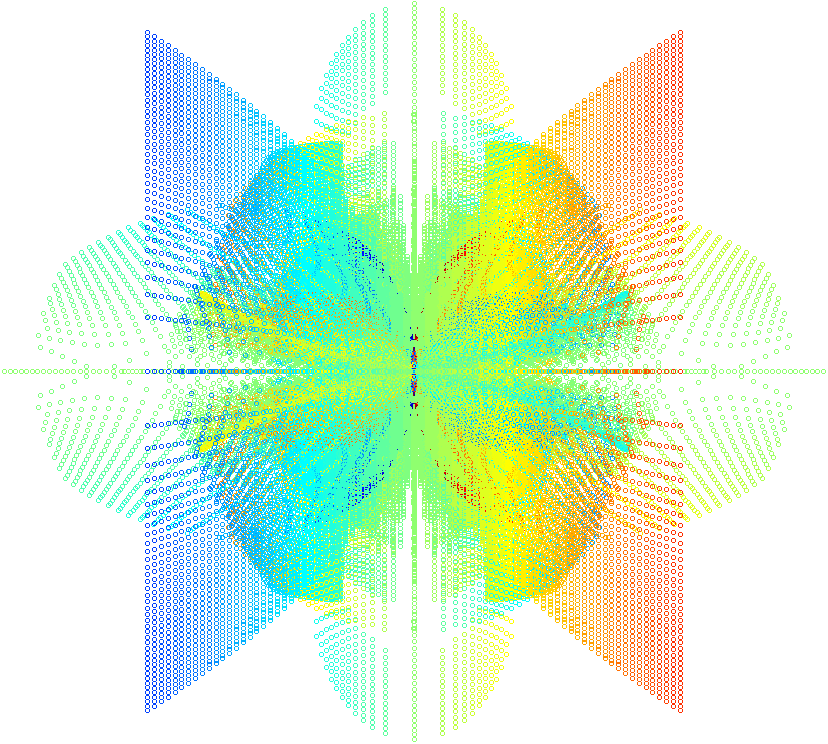
\includegraphics[width = 0.55\linewidth]{monksproj.png}

\end{center}
\null
\vfill
\begin{singlespace}
Manual prepared by\\
Silviana Amethyst\\
 \hfill Manual compiled \today
\end{singlespace}
\newpage





	\tableofcontents
	\eject
	\pagenumbering{arabic} 
	\setcounter{page}{1}
	\eject




\section{Introduction}

The Paramotopy program is a compiled linux/unix wrapper around Bertini 1 which permits rapid parallel solving of parameterized polynomial systems.  It consists of two executable programs: \texttt{Paramotopy}, and \texttt{Step2}, and further depends on having a copy of the parallel version of Bertini 1.  \texttt{Paramotopy} is called from the command line, and in turn calls \texttt{Bertini} and \texttt{step2}.

Briefly, homotopy continuation is the tracking of solutions from one system to another through continuous deformation; a simplified example appears in Figure~\ref{fig:generic_homotopy_continuation}.  Using a combination of prediction and correction, Bertini follows solutions through such a deformation.  First, it obtains the solutions to the initial system.  Taking discrete steps in complex-valued time, each solution path is tracked individually.  If suitable options are chosen in the configuration of the run, precision will be automatically adjusted to compensate for loss of accuracy near system singularities due to poorly conditioned matrices.  Additionally, Bertini has various ``endgame'' schemes for bringing the paths to successful completion, as well as determining whether paths crossed or other problems happened along the way.  Nearly all these options may be accessed through Paramotopy.  For a thorough description of the Bertini 1 program, including many capabilities not used within Paramotopy, see the \href{http://www.nd.edu/~sommese/bertini/BertiniUsersManual.pdf}{Bertini User's Manual}.



Paramotopy is implemented to make use of both the basic zero-dimensional solve Bertini performs by default, as well as exploiting the \texttt{userhomotopy} mode.  An illustration of the scheme is in Figure~\ref{fig:paramotopy_homotopy_continuation}.  First, Paramotopy performs what we define here to be a `Step1' run.  Bertini finds all zero-dimensional solutions to the system supplied to it, for a set of complex parameter values randomly determined; for this solve, there will likely be superfluous paths.  Second, Paramotopy tracks all meaningful solutions found in Step1 (from \texttt{nonsingular\_solutions}) to each parameter point at which the user wishes to solve; this is called `Step2'. Performing the second step in this way will eliminate the extra paths from Step1.  
  
\begin{figure}[h]
\begin{center}
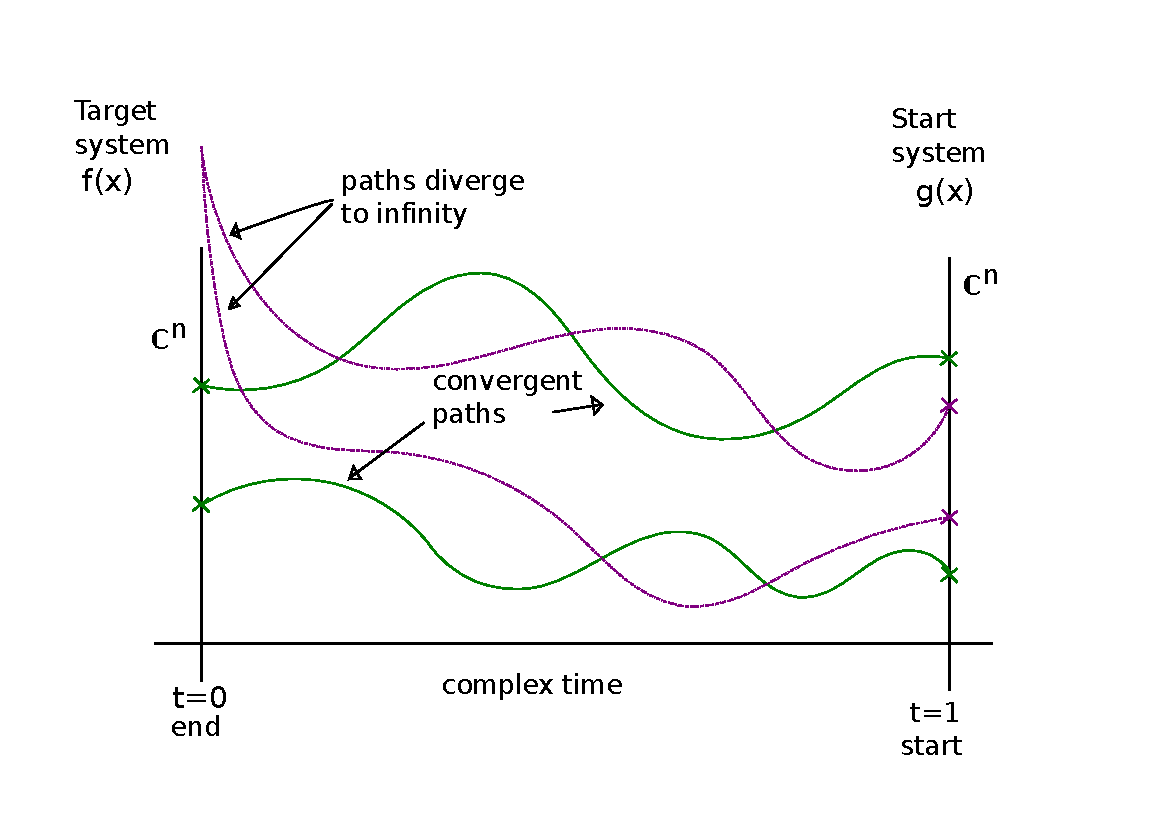
\includegraphics[width=0.65\linewidth]{homotopycontinuation_generic.pdf}
\caption[Generic Homotopy Continuation]{Generic Homotopy Continuation}
\label{fig:generic_homotopy_continuation}
\end{center}
\end{figure}


\begin{figure}[t]
\begin{center}
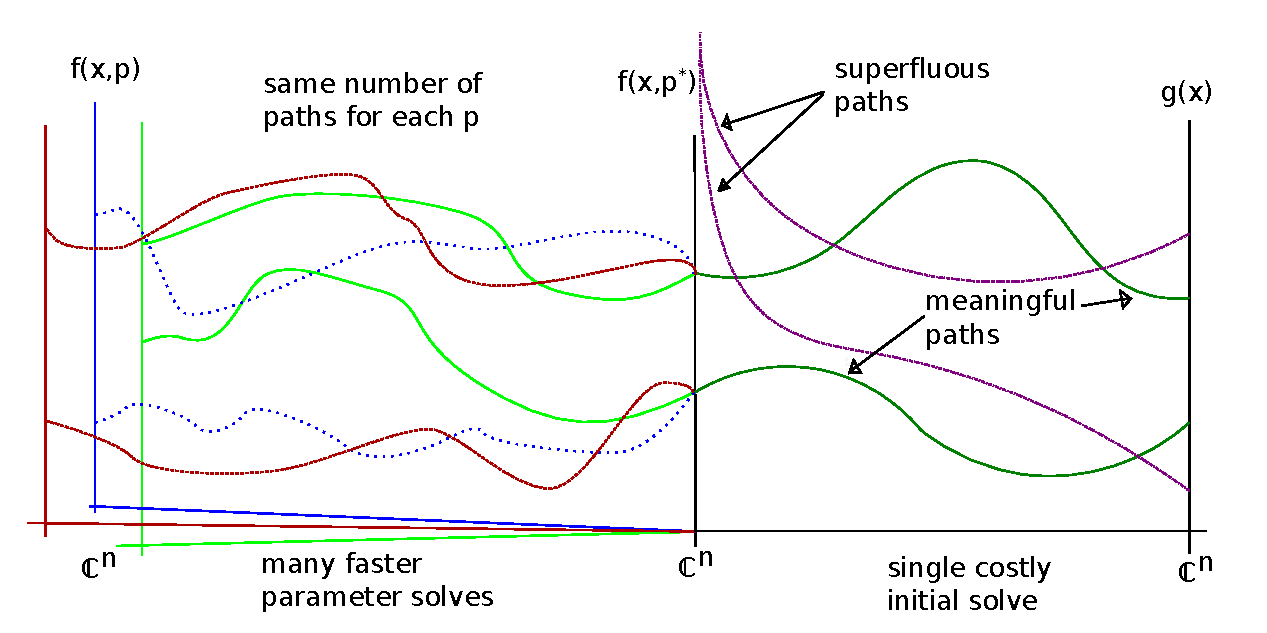
\includegraphics[width=0.9\linewidth]{homotopycontinuation_paramotopy.pdf}
\caption[Parameter Homotopy]{Parameter Homotopy, with initial `Step1' run.}
\label{fig:paramotopy_homotopy_continuation}
\end{center}
\end{figure}

With respect to the soundness and reliability of this method, theory dictates that off a set of measure zero, an algebraic system will have the same number of (complex) roots throughout its parameter space.  Therefore, we are virtually guaranteed that for a \emph{randomly} chosen point in parameter space, we will find the full generic number of solutions.  Then for Step2, as we track from the random point to the specific points at which we wish to solve, we will find all the solutions.

Paramotopy uses a compiled library of Bertini 1, MPICH2 for process distribution, OpenMP for accurate timing measurements, TinyXML for preference and information storage, and Boost for filesystem operations.  System requirements and compilation information may be found in Section~\ref{sec:started}.  In Section~\ref{sec:input} is presented the format for the input files, as well as information on configuring and using Paramotopy.  Specific descriptions of options are given in Section~\ref{sec:options}, and data output is described in Section~\ref{sec:data}.  Coarse troubleshooting tips are in Section~\ref{sec:troubleshooting}.
  




\clearpage

\subsection{Contact}
\label{sec:contact}
For assistance with Paramotopy, please contact Silviana Amethyst at \\
\texttt{silvianaamethyst@gmail.com}.  \\For help with Bertini 1, contact Silviana Amethyst, Dan Bates \\
\texttt{dbates@usna.edu}, \\or one of the other Bertini 1 authors.

\subsection*{Acknowledgements}
\begin{itemize}
\item  This research utilized the CSU ISTeC Cray HPC System supported by NSF Grant CNS-0923386.
\item  This material is based upon work supported by the National Science Foundation under Grants No. DMS-1025564 and DMS-1115668.
\end{itemize}

The authors wish to thank the following:
\begin{itemize}
	\item Boost,
	\item \href{http://www.bedaux.net/mtrand/}{MTRand},
	\item Zube,
\end{itemize}

\clearpage
\subsection{License}
\label{sec:license}
Paramotopy is free, open source software with restrictions.  The license is available on the web at \href{https://paramotopy.com/resources/programs/paramotopy_license.txt}{paramotopy.com}.

\subsection*{Disclaimer}
Paramotopy and all related code, executables, and other material are offered without warranty, for any purpose, implied or explicit. 

Any opinions, findings, and conclusions or recommendations expressed in this material are those of the author(s) and do not necessarily reflect the views of the National Science Foundation.




\clearpage
\section{Getting Started}
\label{sec:started}

\subsection{Compilation and Installation}

Paramotopy has the following library dependencies: 
\begin{itemize}
\item \href{http://sourceforge.net/projects/tinyxml/}{Tinyxml}  (lies internally to the program's folders, as per the license agreement).
\item MPICH2,
\item  \href{http://www.boost.org/}{Boost} -- regex, system, filesystem (for file manipulation), and a few others.  Make sure you have the entire boost library.  Minimum version is 1.53.
\item OpenMP (for the most accurate timing available).  Seems standard on *nix variants these days.
\item \href{http://www.bedaux.net/mtrand/}{MTRand} (lies internally to the program's folders, as per the license agreement)
\end{itemize}
\noindent For installation of dependencies on a Mac, consider using \href{http://mxcl.github.io/homebrew/}{Homebrew}.
\vspace{10mm}

\noindent In addition, Paramotopy relies on a suitably compiled version of Bertini 1, which has the following dependencies:
\begin{itemize}
\item \href{http://www.mpfr.org/}{mpfr} 
\item \href{http://gmplib.org/}{gmp}
\item Bison
\item Flex
\item MPICH2
\end{itemize}


Paramotopy is built using the Autotools.  If you cloned the repo from Github, you should 
\begin{itemize}
\item {libtoolize \&\& autoreconf -vfi} in the directory first, if on Linux
\item {autoreconf -vfi} in the directory first, if on Mac
\end{itemize}
Then, use the standard {\tt ./configure}, {\tt make}, {\tt make install} pattern.  

You may have to add the path to where you installed the Bertini libraries to {\tt LD\_RUN\_PATH} and {\tt LD\_LIBRARY\_PATH}, especially if you customized {\tt prefix} when installing Bertini 1.


\clearpage
\subsection{Using Paramotopy}
\label{sec:running}

\begin{figure}[h]
\begin{center}

\includegraphics[scale=\screencapsize]{welcome.png}
\caption[Welcome Screen]{The welcome screen.  If you do not supply the filename as the first argument to Paramotopy from the command line, it will immediately prompt you for the name.  You cannot use the program without an input file.}
\label{screen:welcome}
\end{center}
\end{figure}



\begin{figure}[h]
\begin{center}
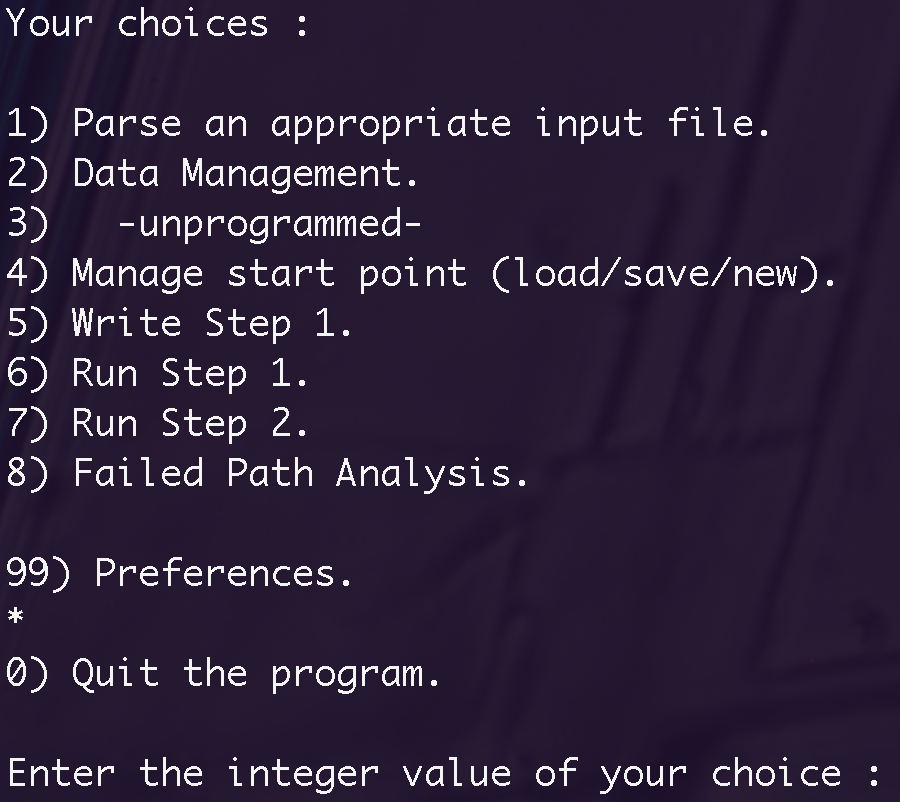
\includegraphics[scale=\screencapsize]{mainmenu.png}
\caption[Main Menu]{Main menu, describing the available choices.  Use numeric input, or whatever it prompts for. If you just loaded the program, it will describe what directory it is working in.}
\label{screen:mainmenu}
\end{center}
\end{figure}



\clearpage
\section{Input Files}
\label{sec:input}

\index{main menu option 1}\index{input file format}The input file format for Paramotopy is fairly simple.  Extra white space on a single line is acceptable, but there must be no extra blank lines.  Illustrative examples appear in Files \ref{genericinput},\ref{bioinput},\ref{roboinput}. The input file consists of:

\begin{enumerate} 
\item Declare the numbers of: functions (\texttt{a}), variable groups (\texttt{b}), parameters (\texttt{c}), and constants (\texttt{d}), in one line, separated by spaces; e.g. \begin{center} \texttt{a b c d} \end{center}
\item Functions declaration, without any name declarations or terminating semi-colons.  
\item Variable groups come next, with each group getting its own line; variables are comma separated, and there is \emph{no terminating character}.  
\item Constant declaration,  with the word \texttt{constant} appearing before a comma separated, semi-colon terminated line containing the constant names.  Each constant gets its own line, with \texttt{name = value;} being the format.  
\item Finally, the type of solve is indicated: 
\begin{itemize} 

	\item 0 \index{computer generated mesh}indicates the computer will supply a mesh.  The final lines tell the name of each parameter, starting point of discretization, ending point of discretization, and number of discretization points.  The format for a line of parameter declaration is \begin{center} \texttt{name  a  b  c  d  e}, \end{center} where startpoint = \texttt{a}$+$\texttt{b}$i$, endpoint = \texttt{c}$+$\texttt{d}$i$, and \texttt{e} indicates the number of discretization points, which must be an integer. See File \ref{bioinput}.

	
	\item 1 \index{user-defined parameter files}asserts the user supplies a text file containing parameter values; the next line is the name of the file, and the final lines simply indicate the parameter names.  See File \ref{roboinput}.
		\end{itemize}
\end{enumerate}

\File{Generic Paramotopy input file.}{genericinput}{genericinput.para}


Paramotopy has minimal error correction in this portion of the program, so an error in an input file is likely to cause a fairly benign (will not corrupt data) program crash.  If the program is able to parse the input file without errors, it will display information to the screen and the user may check everything has been imported correctly.  More syntax checking will be added later.



\File{Paramotopy input file demonstrating use of computer-generated mesh, and constant declaration.  Line 1 indicates 7 equations (lines 2-8), in 1 variable group (line 9), with five parameters (lines 33-34), and 21 constant declarations (10-31).  On line 32, \texttt{0} tells Paramotopy to make a mesh from the parameters discretized in lines 33-34.  Parameter \texttt{k4} will be broken into 40 points on the complex line segment $0+0i$ to $1+0i$.  Similarly, \texttt{k2} will be broken into 50 points, so a solve using this input file would have 2000 points total in the Step2 run.}{bioinput}{bioinput.para}

\File{Paramotopy input file demonstrating use of user-defined parameter file.  Line 1 indicates 12 equations (lines 2-13), in 1 variable group (line 14), with five parameters (named on lines 17-21), and zero constant declarations. Line 15's \texttt{1} indicates Paramotopy should look for the file on the next line, titled \texttt{robomc\_10000}.  The name of the file is arbitrary, but should be at the same path at the input file.  The parameters are named \texttt{a}, \texttt{delta}, \texttt{x}, \texttt{y}, \texttt{z}.  }{roboinput}{roboinput.para}






\clearpage

\subsection{Monte Carlo Input}

Paramotopy enables the user to supply their own plain text file of parameter points over which to solve a parametrized family of polynomials.  The first line is an integer indicating the number of parameter points.  The remainder of the file gives the actual parameter values, as one point per line, with parameter real-complex pairs separated by spaces.  See File \ref{roboinput} for an example of such a Paramotopy input file, and File \ref{robomc} for an example of the user-defined file. \index{monte carlo samplings}\index{user-defined parameter files}


\File{User-defined parameter point file.  This file is named in the input file (this  is \texttt{robomc\_10000}, as mentioned in File \ref{roboinput}, and must be placed in the same directory (doing otherwise is untested).  The first line of the file must be an integer indicating the number of parameter points which follow, in this case 10000.  This integer must be at most the number of parameter points in the file, though it can be fewer. For the remainder of the file, each line indicates one parameter point, and each real-complex pair is separated by a space. }{robomc}{robomc.para}


















\clearpage
\section{Options \& Configuration}
\label{sec:options}

\index{preferences location}Persistent configuration of Paramotopy is maintained through the {\begin{center}\texttt{\$HOME/.paramotopy/paramotopyprefs.xml} \end{center}} \noindent file located in the home directory.  The following sections describe what the settings affect.  Note that since the preferences file is merely text, the user could manually hack it with a text editor.


\begin{figure}[h]
\begin{center}
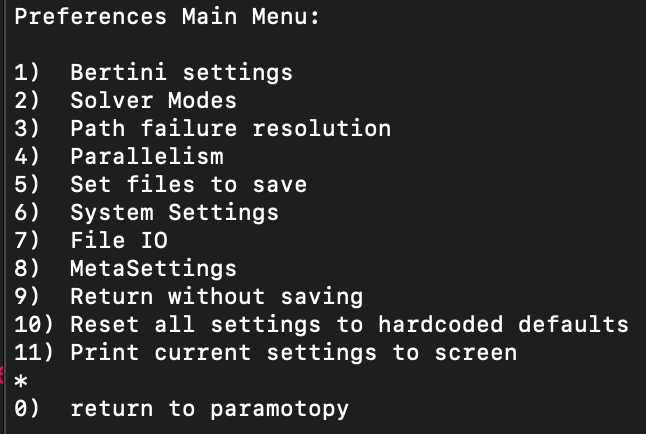
\includegraphics[scale=\screencapsize]{preferencesmainmenu.png}
\caption[Preferences Main Menu]{The Paramotopy main menu.  Interaction is via mainly numeric input at the console.}
\label{screen:prefsmainmenu}
\end{center}
\end{figure}


\subsection{Step1 and Step2 Bertini Settings}

Separate settings categories are present for both the Step1 and Step2 runs, and persist from run to run, and session to session.  These are written directly into the input files for Bertini, and there is no error checking -- if the user sets a setting to one disallowed, or misspells a name, the Bertini calls in Step1 or Step2 will just ignore the setting.

\begin{figure}[h]
\begin{center}
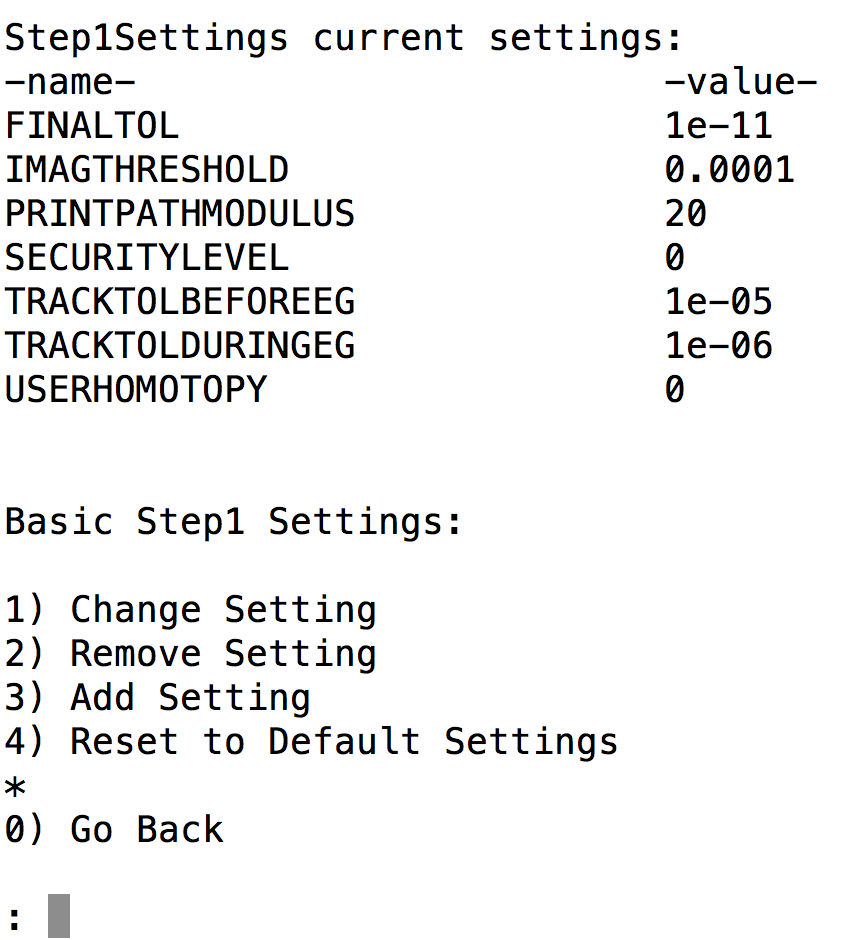
\includegraphics[scale=\screencapsize]{step1settings.png}
\caption[Step 1 Settings]{\index{bertini settings}Step1 Settings.  All settings are direct Bertini config options.}
\label{screen:step1menu}
\end{center}
\end{figure}

%\begin{figure}[h]
%\begin{center}
%\includegraphics[scale=\screencapsize]{step2settings.png}
%\caption[Step 2 Settings]{\index{bertini settings}Step2 Settings. All settings are direct Bertini config options.}
%\label{screen:step2menu}
%\end{center}
%\end{figure}

Options are to change, delete, and add a setting.  User may also reset all of that Step's settings, and reset to default, which are the Bertini default values as well.  Note that each setting has a type, being either a string, integer, or double value.  Doubles may use the \texttt{1e-4} format for convenience.  While capitalization does not matter in Bertini, Paramotopy is currently case-sensitive, so deleting or changing a setting requires the same capitalization as displayed.




\subsection{Solver Modes}


\begin{figure}[h]
\begin{center}
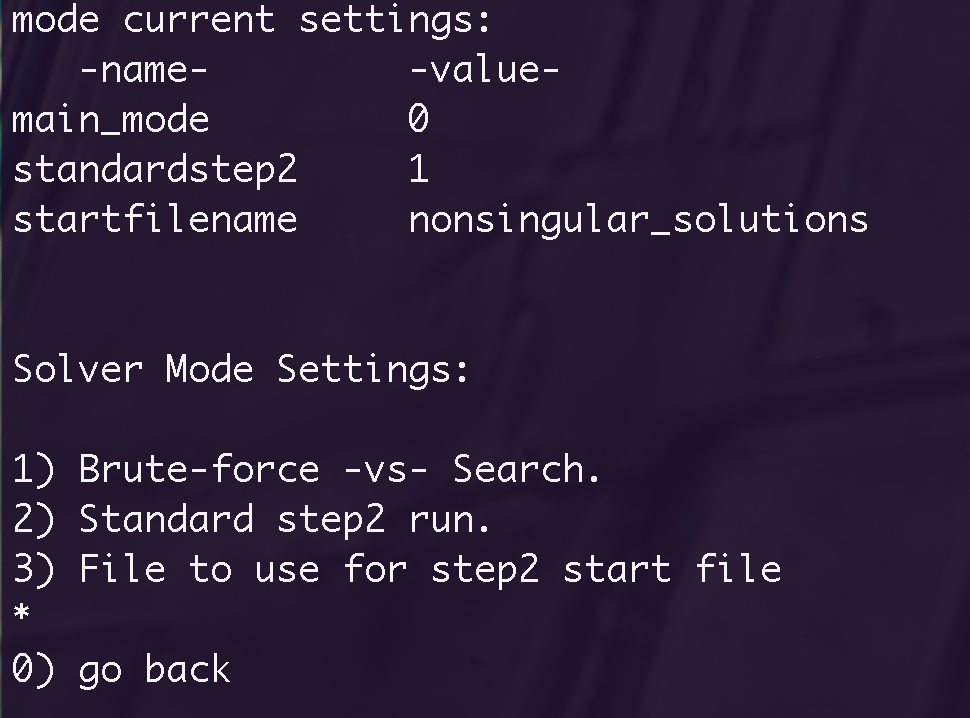
\includegraphics[scale=\screencapsize]{modemenu.png}
\caption[Solver Mode Menu]{\index{mode menu} Choose from a suite of modes, and configuration options.}
\label{screen:modemenu}
\end{center}
\end{figure}



\begin{itemize}
	\item  {\tt Brute-force -vs- Search}  \\ choose whether to solve across the mesh or sampler you feed in, or to search for solutions with a particular property.
	\item {\tt Standard step2 run.} \\ choose to run a total-degree solve each parameter point, or use coefficient parameter homotopy as usual.
	\item \texttt{Set the file to use for step2 start file} \\ \index{start file}User may select to use either the \texttt{nonsingular\_solutions} or \texttt{finite\_solutions} output from Step1 as the start file for Step2 solves.
\end{itemize}

\subsection{Path Failure}

\begin{figure}[h]
\begin{center}
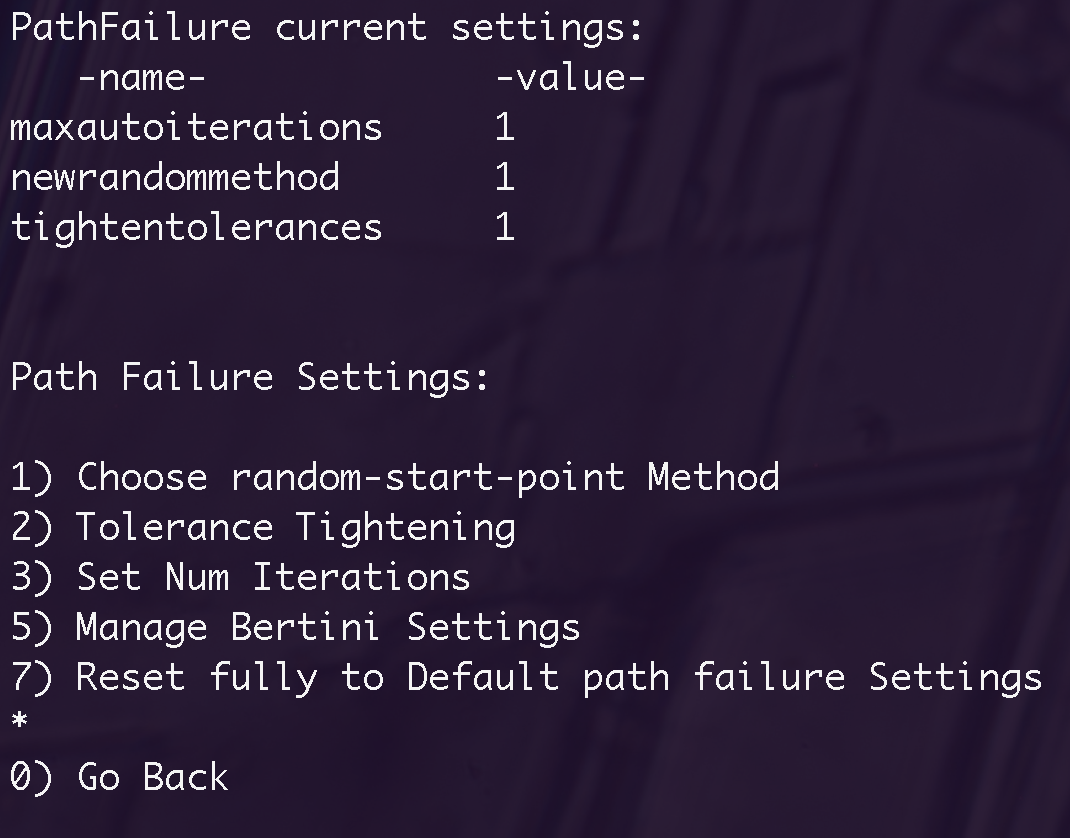
\includegraphics[scale=\screencapsize]{pathfailuresettings.png}
\caption[Path Failure Settings]{\index{failed paths menu}Path Failure Settings menu.  The path failure analysis section of the program utilizes the Bertini preferences from the Step1 and Step2 sections, optionally changing them with successive runs.}
\label{screen:pathfailuremenu}
\end{center}
\end{figure}

\begin{figure}[h]
\begin{center}
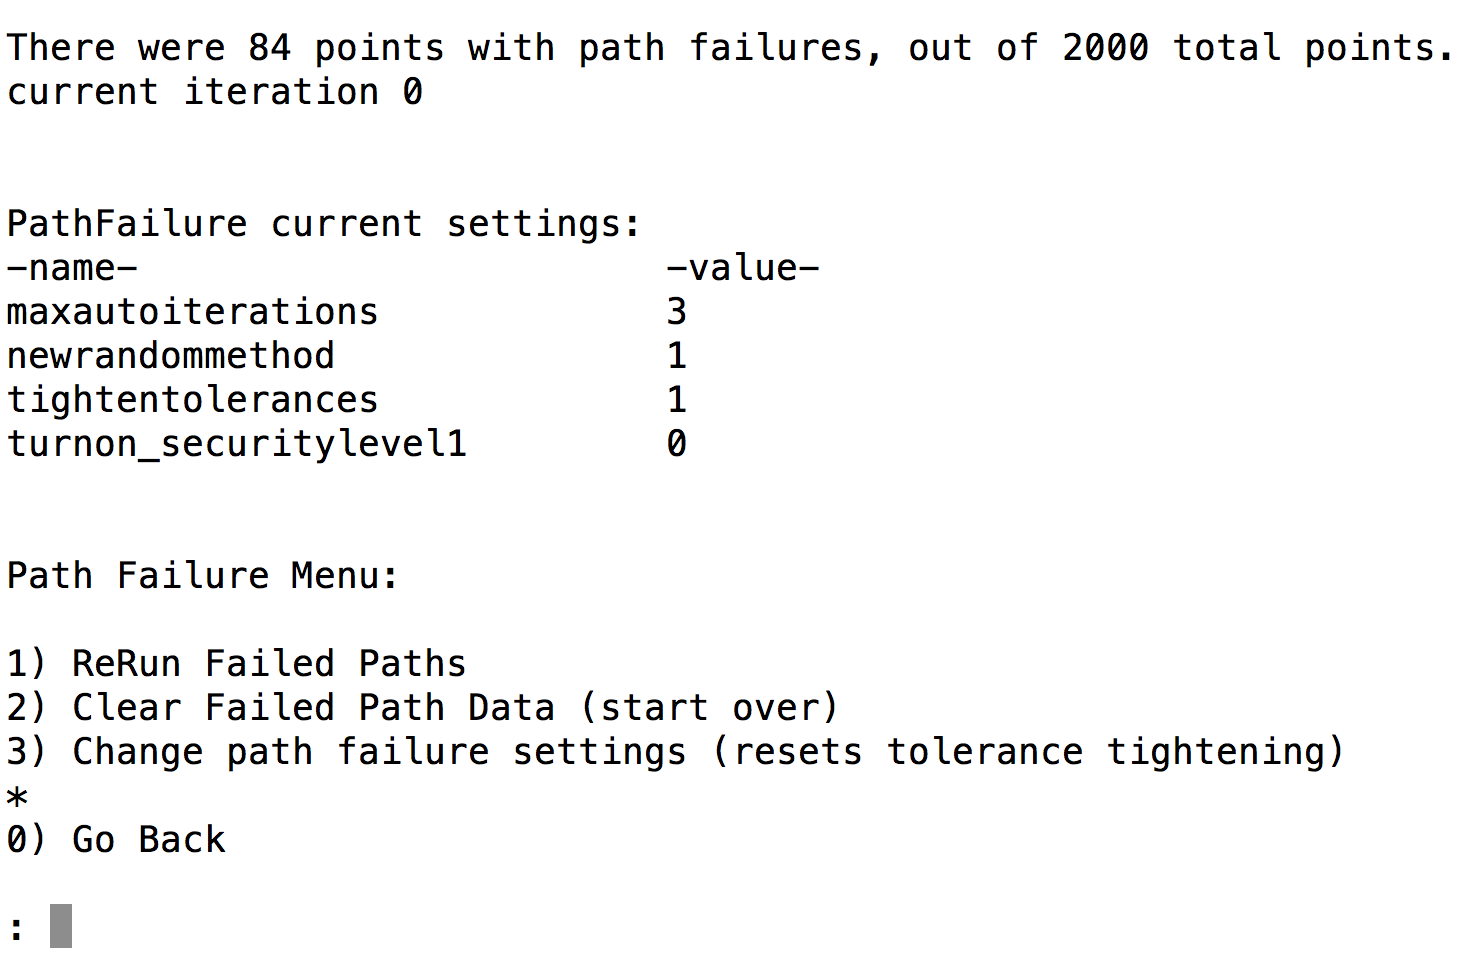
\includegraphics[scale=\screencapsize]{failure.png}
\caption[Path Failure Re-solve Menu]{\index{failed paths menu}Path Failure Re-solve menu.  User can continue to attempt to re-solve, adjust settings, and delete files and start over.}
\label{screen:failure}
\end{center}
\end{figure}

\index{failed path analysis}Paramotopy detects failed paths that occur during a run, and has methods for resolving the system, repeatedly if necessary, to get the proper solution set. 

\begin{itemize}
	\item \texttt{Choose random-start-point Method} \\ When resolving points with failed paths, Paramotopy can optionally choose a new start point before solving the set of fails.  To be developed is a variety of methods for choosing this start point; {\em e.g.} specifying a distance from the original start point, etc.
	\item \texttt{Change security level} \\ ensure \texttt{securitylevel=1} is turned on, for more secure solution of failed paths.
	\item \texttt{Tolerance Tightening} \\ When Failed Path Analysis is entered in Paramotopy, the settings are those currently used for Step2 runs.  If tolerance tightening is enabled, at each iteration of resolve, the \texttt{finaltol}, \texttt{tracktolbeforeeg}, and \texttt{tracktolduringeg} values are decreased by a factor of ten.  
	\item \texttt{Set Num Iterations}  \\ Path Failure mode will automatically try  to re-solve failed paths [up to] this number of times before returning back to the user for input.
	\item \texttt{Reset to Default Settings} \\ Reset PathFailure settings to default hardcoded values.
\end{itemize}

\clearpage






\subsection{Parallelism}
\index{parallelism preferences}Parallelism is achieved using MPICH2.  Paramotopy itself acts as a gateway to the Step2 program, where all the real work is done.  The gateway allows the user to load input files, make new data folders, change settings, run Bertini for Step1, call Step2, and perform Failed Path Analysis on a completed Step2 run.  The gateway model was used because Bertini uses MPI itself, and \texttt{MPI\_Init()}, \texttt{MPI\_Finalize()} can only be called once within a program.  Therefore, Step2 uses the nonparallel version, whereas Step1 can call either one.

\begin{figure}[h]
\begin{center}
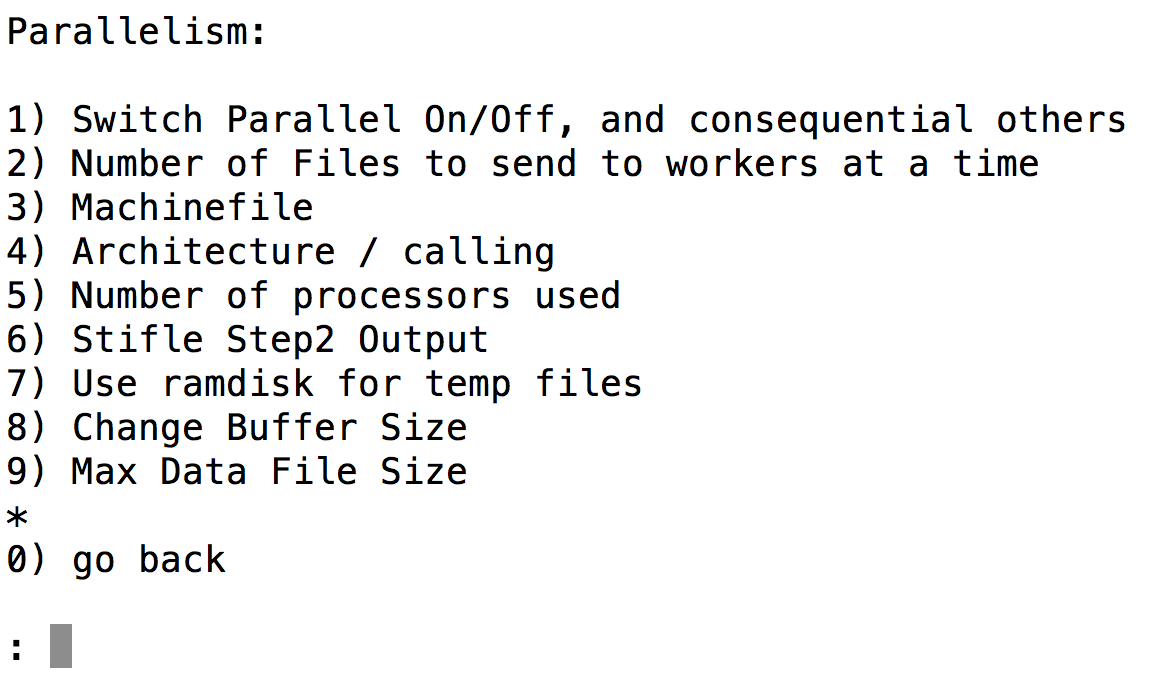
\includegraphics[scale=\screencapsize]{parallelmenu.png}
\caption[Parallelism Menu]{Parallelism menu.}
\label{screen:parallelmenu}
\end{center}
\end{figure}

\begin{itemize}
	\item \texttt{Switch Parallel On/Off}  \\turn on or off parallel solve mode.  If off, then a single processor will be used for all portions of the program
	
	\item \texttt{Number of Files to send to workers at a time}\\ \index{file distribution}to minimize network traffic, it is advisable to distribute the work in chunks.  Setting this value close to one will kill performance, while setting it near the total number of parameter points will send all the work to a single processor.  It is up to the user to find balance, though one rule of thumb would be to set this to:   \\ \hspace{2in} (total\#files /($k \times $\#processors) ), \\with $k$ perhaps 5 or 10, meaning that 5 or 10 batches would be sent to each processor throughout the computation.
	
	\item \texttt{Machinefile} \\ \index{machinefile}some MPI installations require a machine file for process distribution.
	
	\item \texttt{Architecture / calling} \\ set the call to start an MPI process on your machine.  Two defaults are built in: \texttt{mpiexec}, \texttt{aprun}.  You may also use your own, although there is no error checking for whether your custom command exists, or functions properly.  We will soon add the feature of custom calling sequences for more complex command strings.
	
	\item \texttt{Number of processors used} \\ Set the number of processors for Step1, Step2, and rerunning of failed paths (realized as Step2 runs).  There should be at least two processors for this mode, as Paramotopy currently uses the controller-worker model, with a single controller.  If you wish to use only one process, switch off parallel mode.  
	


\end{itemize}


\subsection{File Saving}


\begin{figure}[h]
\begin{center}
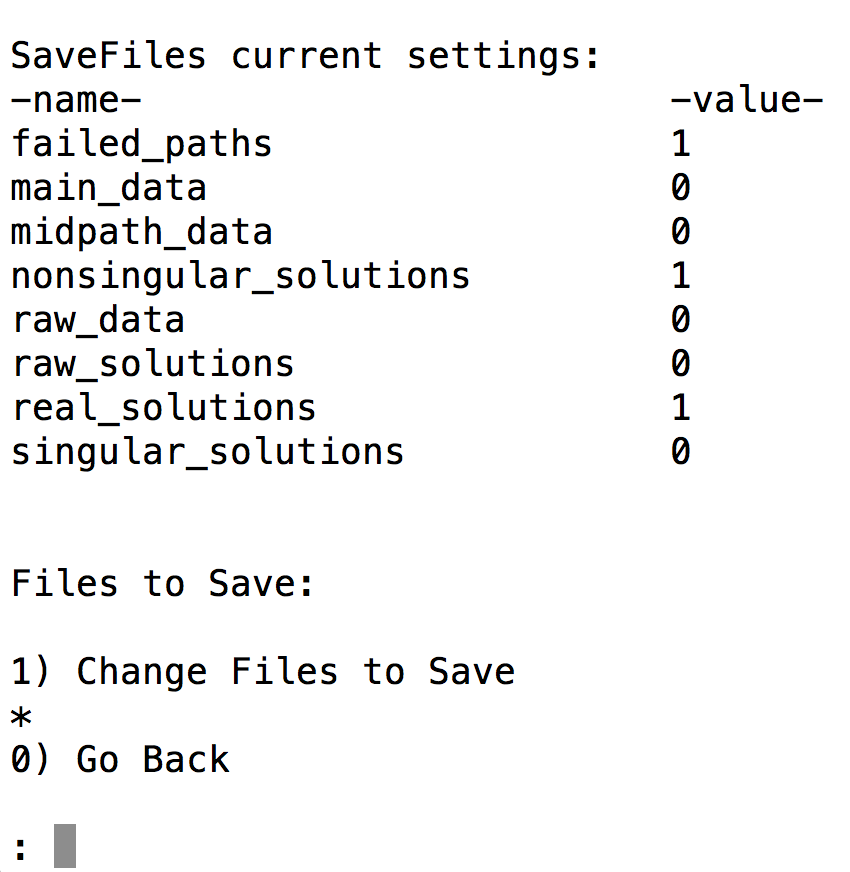
\includegraphics[scale=\screencapsize]{savefiles.png}
\caption[File Saving]{Paramotopy can save each of the output files from Bertini, for each point at which it solves the input system.  \texttt{failed\_paths} is always saved; the rest are optional.}
\label{screen:savefilesmenu}
\end{center}
\end{figure}

\index{choosing saved files}Bertini produces several output files which may be desirable to keep.  The file named \texttt{failed\_paths} is always saved, to enable Failed Path Analysis.  All other files are optional.  Some are more useful than others for humans or computers.  For a more thorough description of the output of Bertini, see the \href{https://www.nd.edu/~sommese/bertini/BertiniUsersManual.pdf}{Bertini User's Manual}.







\subsection{System Settings}
\begin{figure}[h]
\begin{center}
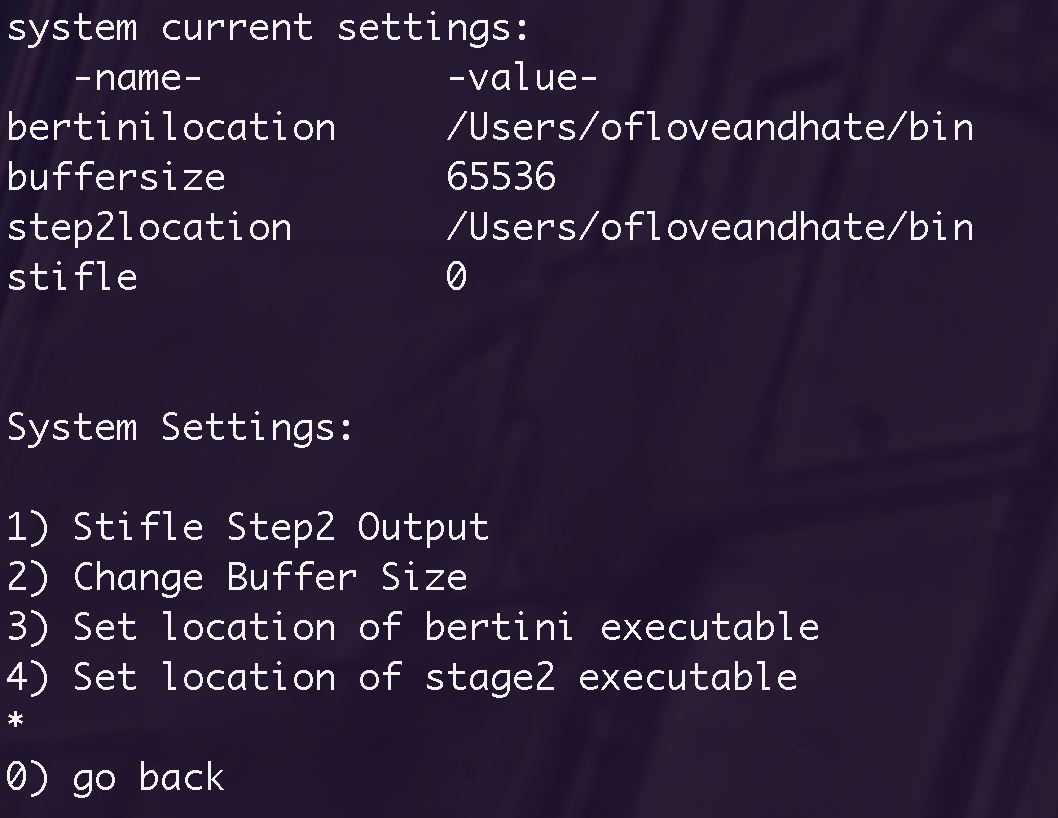
\includegraphics[scale=\screencapsize]{systemmenu.png}
\caption[General Settings Menu]{\index{general settings menu}System Settings menu.}
\label{screen:systemmenu}
\end{center}
\end{figure}

\begin{itemize}

	\item \texttt{Stifle Step2 Output} \\ \index{stifle output}Bertini produces an overwhelming amount of screen output.  Not only is this annoying, but sending text to the screen overwhelms the network.  It is suggested to stifle only when you are confident in the success of your Step2 runs.  Stifling by redirection to \texttt{/dev/null} produces a significant speedup.
	
	\item \texttt{Change Buffer Size}\\ \index{read buffer}to minimize writes to the hard drive, each worker buffers its files in memory, and writes to disk only when a threshold is reached.  To change this threshold, change this buffer size.
	
	\item \texttt{Manually set location of bertini executable} \\ \index{\texttt{bertini} location}Paramotopy automatically scans the current directory (\texttt{./}) and \texttt{\$PATH} for Bertini at startup, in that order, and chooses the first instance of Bertini it finds.  If the user wishes to manually change the location for Bertini, they should this option.
	
	\item \texttt{Manually set location of step2 executable} \\  \index{\texttt{step2} location}Same as for Bertini.
	
	
\end{itemize}




\subsection{FileIO}
\label{sec:fileIO}

\begin{figure}[h]
\begin{center}
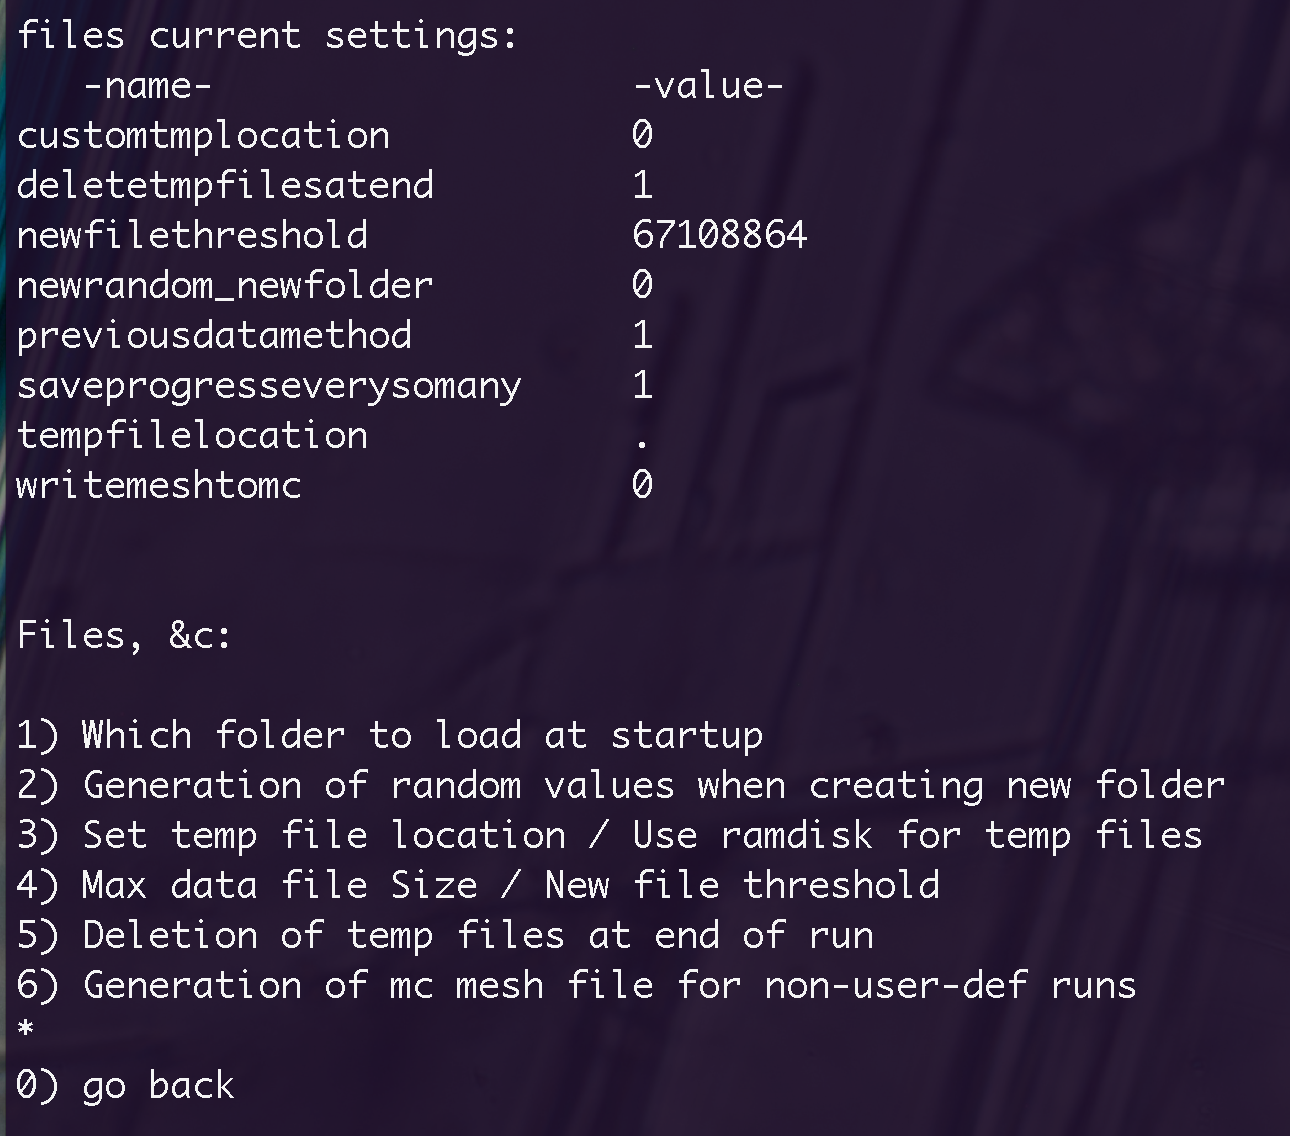
\includegraphics[scale=\screencapsize]{fileIOmenu.png}
\caption[File IO Menu]{\index{file I/O menu}File IO menu.}
\label{screen:fileIOmenu}
\end{center}
\end{figure}

\begin{itemize}
	\item \texttt{Load Data Folder Method} \\ \index{restoring previous runs}At launch of Paramotopy, if not supplied with an argument of the filename to load, Paramotopy will ask the user for the filename.  Each filename gets its own folder for storing data, and in this folder will be another folder containing the data for a run.  At launch, Paramotopy will do one of the following:
		\begin{itemize}
			\item Reload data from the most recent run,
			\item Make a new run folder, and make new start point,
			\item Ask the user what to do.
		\end{itemize}
	\item \texttt{Generation of random values at new folder (during program)} \\ \index{new run folders}If, while running the program, the user wishes to start a new run, should Paramotopy:
		\begin{itemize}
			\item Keep the random values currently in use, or
			\item Make a new set of random values.
		\end{itemize}
	\item \texttt{Set temp file location / use ramdisk for temp files} \\ \index{ramdisk}\index{temp files}Bertini uses hard disk IO to communicate with itself and other processes.  This can overwhelm the hard disk, uses read/write cycles reducing the lifetime of a hard drive, and injures performance.  Using a location in memory as a hard disk, otherwise known as a ramdisk, will grant you enormous performance gains.  Two locations are scanned for existence by default: \texttt{/dev/shm} and \texttt{/tmp}.  If either are found, the user is prompted for confirmation.  The user may also choose a custom location.  However, at present time the name of the temporary file location root directory must be the same across all computers used.  Note: Paramotopy does not guarantee that the chosen location is usable in the desired fashion; the user must ensure that the temporary location is read/writable.
	
	
	
	\item \texttt{Max Data File Size} \\ \index{data file size}The text files produced by Paramotopy grow in time, of course.  To ensure that you don't produce unwieldly files, change the maximum file size for data files.  The default is 64MB.  This maximum is not a \emph{hard} maximum, in the sense that a new file is started only after the max is achieved.
	
	\item \texttt{Deletion of tmp files} \\ \index{temp files}Step2 involves creation of many temporary files.  Each worker creates a folder in which to initialize Bertini, named \texttt{init*}, where \texttt{*} is the id number assigned by MPI.  Then, each worker creates another folder named \texttt{work*} with the same naming scheme, in which it produces the data.  All Bertini data is created in this folder.  Switching this settings will toggle whether these folders ought to be deleted at the end of a successful run.
	
	\item \texttt{Generation of mc mesh file for non-user-def runs} \\ \index{\texttt{mc} mesh file}User can choose whether \texttt{step2} ought to create a text file containing all the parameter values for all points, during a computer-generated mesh run.  This file is usable in a user-defined run.  However, this file can be very large, and eats hard drive write throughput, so we have provided the option to not create this file.
	
	
\end{itemize}


\subsection{Meta Settings}
\label{sec:meta}

\begin{figure}[h]
\begin{center}
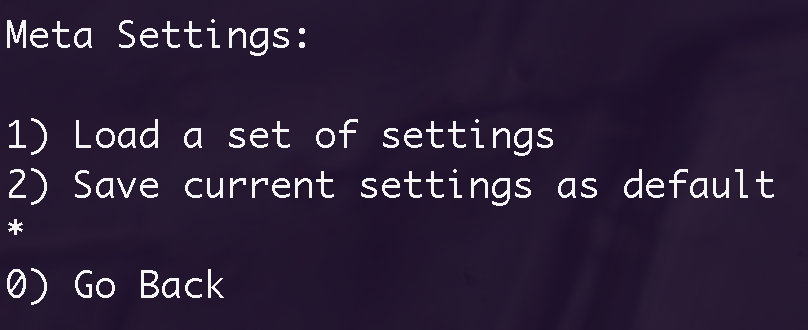
\includegraphics[scale=\screencapsize]{metamenu.png}
\caption[Meta Menu]{\index{meta settings}Meta Settings menu.}
\label{screen:metamenu}
\end{center}
\end{figure}


\begin{itemize}
	\item {\tt Load a set of settings} \\ Scans {\tt \$(HOME)/.paramotopy} for {\tt .xml} files for settings, and offers you a choice to load.
	\item {\tt Save current settings as default} \\ Saves what you have in memory for settings, right now, as the default for future filenames.
\end{itemize}

\clearpage
\section{Data Gathering}
\label{sec:data}

\index{data gathering}Paramotopy is capable of producing immense amounts of data.  Probably the two most useful files you can choose to save are \texttt{nonsingular\_solutions} and \texttt{real\_solutions}.  Both are easy to have a machine parse, with predictable numbers of lines per parameter point.

At some points in parameter space,  polynomial systems  will be faster to solve than others.  Combined with the use of a parallel machine, this will result in data files which are out of order.  Whatever data collection method you use, you must deal with this fact.

Data collection is achieved by simply copying the Bertini output file into memory, and then, along with the index of the parameter point and the parameter values, into a collective output file.  The format is essentially what appears in File~\ref{output}:

\File{\index{data file format}Example output file from Paramotopy.  The first line of each file created by Paramotopy declares the names of the parameters.  Each parameter point gets its own section, with the index (lines 2, 12), parameter values (lines 3, 13), and copied Bertini output.  This is an example of \texttt{real\_solutions} output, so lines 4,14 indicate the number of solutions which follow.  The actual solutions appear as well.  Note that lines 4-10, and 14-20, are unmodified Bertini output, complete with whitespace.}{output}{output.para}

\index{main menu option 2}Paramotopy has a method implemented in \texttt{Data Management} which gathers and orders the data produced in a run, as well as incorporating the re-solved data generated in Failed Path Analysis.  Note that this method so far only gathers \texttt{failed\_paths} and \texttt{*\_solutions} data file types.  The others have yet to be implemented.  The data gathering requires, but does not check for, free disk space available for at least the amount occupied by the generated data in \texttt{bfiles\_filename/run*/step2/DataGathered/c*}.


The author Silviana Amethyst has some generic \textsc{Matlab} code which can do basic parsing of some file types, as well as data display methods.   If you need help with any aspect, don't hesitate to ask! Contact info in Section \ref{sec:contact}.







\clearpage
\section{Troubleshooting, Known Problems}
\label{sec:troubleshooting}

\begin{itemize}
	\item Step1 fails 
		\begin{itemize}
		\item Are all the settings properly spelled, and allowed?
		\item Was the calling sequence correct?
		\item Do you have the \emph{parallel} version of Bertini installed?
		\item Try running Bertini on the created input file.
		\end{itemize}

	\item Step2 fails
		\begin{itemize}
		\item Are all settings spelled properly and allowed?
		\item Was the calling sequence correct?
		\item Did Paramotopy correctly parse your input file?
		\item Did the temporary files write to an acceptable location?
		\item Try running Bertini on the created input file. $\rightarrow$ Bertini might provide a useful error report.
		\item Turn off stifling of output, so that you can read any generated error messages.
		\end{itemize}
\end{itemize}


A list of known problems:
\begin{itemize}
	\item There cannot be any spaces in folder or input file names.  
	
\end{itemize}

\ifx\standalonemode\undefined

\else
	\begin{singlespace}
	\bibliographystyle{ieeetr}
	\bibliography{bibliobiblioparama}
	\end{singlespace}
	
	\begin{singlespace}
	\printindex
	\end{singlespace}
\fi